\chapter{Methodology}
\setcounter{footnote}{0}
\label{ch:methodology}
What methods do we use to get answers to the questions asked? How can we ensure that the research is reliable? These are the questions this chapter will answer.

\section{Research design}
\label{sec:researchquality}
We need answers to the following questions before we can start with our research. What is the reliability we pursue, and how do we reach this reliability? What methods do we have for our research, and which ones do we use? What is our research model? We will design our reliability with support of quality attributes and principles. Secondly, we will briefly explain possible research methods before beginning a high-level design. We close this section with our choice of research method and how we think we can comply with the quality attributes to meet our reliability expectations.

\subsection{Research quality}
\label{sub:researchquality}
We increase the rigorousness of the research by applying quality principles by applying four principles. These principles are replicability, independence, precision and falsification \parencite[p.~16--18]{Recker2012}. Replicability makes sure that a third party can repeat the research, while independence frees the research from subjective judgement. Precision assures that all the concepts, constructs, and measurements allow others to use, apply and challenge those concepts, constructs and measurements. Falsification implies that the research results can be disproven.

We find replicability and reusability essential. We believe that the results of this research should be open and available for everyone. We adopt the FAIR principles \parencite{Wilkinson2016} to support us in achieving this replicability and reusability. FAIR stands for findability, accessibility, interoperability, and reuse of digital assets. Findability assures that research data, and metadata is easy to find for both humans and computers. Accessibility is that it can also be accessed when the data is found. Interoperability is about that data must support integration with other data. The last principle is reusability. With reusability, the data and metadata are well described for combining and replicating.

\subsection{Research method}
\label{sub:researchmethods}
The most popular research methods are either quantitative or qualitative \parencite[p.~65]{Recker2012}. A quantitative method uses techniques to answer a research question emphasising using quantitative data \parencite[p.~66]{Recker2012}, it has its focus measurement \parencite[p.~88]{Recker2012}, while a qualitative method is about assisting researchers in understanding a phenomenon in context. ''Qualitative research is for exploratory research where a phenomenon is not yet fully understood, not well researched, or still emerging'.' \textcite[p.~84]{Recker2012}. With qualitative research, the focus is on text rather than numbers. Qualitative research is about what people have said, done, experienced or believe. Qualitative methods are case study research, action research, grounded theory, and others. A case study is a detailed study of a specific subject, such as a person, group, place, event, organisation, or phenomenon \parencite[p.~95]{Recker2012}. Grounded theory is about collecting data in order to develop new theories \parencite[p.~102]{Recker2012}. Action research introduces changes and interventions into a context and studies the effects \parencite[p.~99]{Recker2012}.

\subsection{Triangulation}
\label{sub:triangulation}
Stating something by only using one method is not reliable. The result can be biased or can be coincidental. The result will get better if it is validated by multiple methods. This validation method is called \gls{triangulation}. ''\Gls{triangulation} means seeking convergence and corroboration of results from different methods and designs studying the same phenomenon'' \parencite[p.~110]{Recker2012}. Using different sources for cross-validation strengthens the findings to be more reliable and valid. The researcher gains a more nuanced picture of the situation by doing so \parencite[p.~88]{Recker2012}. Triangulation increases the validity, credibility, and authenticity of research data, analysis and interpretation. \Gls{triangulation} can be used in quantitative as well as qualitative methods \parencite[p.~88]{Recker2012}. \Gls{triangulation} will increase the validity of research results.

\subsection{Research model}
\label{sec:researchmodel}
The topic of \gls{antifragile} is still relatively young, and as far as we have been able to find, it has not been used in practice yet in the context of systems. Let alone with a \gls{sos}, the Dutch public sector. Little information is therefore available to perform a quantitative analysis. The chosen research method is qualitative. This method focuses on what people said, done, believed or experienced. The research approach explores and develops generalised success factors for \gls{antifragility} in the \gls{ps}. The research focuses on a relatively new research domain, is emergent and lacks a substantive theory. This information indicates that the research has a base attitude of the qualitative method, particularly Grounded Theory. The challenge of this method is the validation of the results. How can we ensure that we have done everything to remove possible subjectivity? Using the triangulation method, we minimise possible subjectivity by using multiple research tools and different sources.

So how do we apply the qualitative research method with triangulation? We are searching for an answer to the research question 'What are the success factors that positively influence the contribution of \acrlong{ea} in achieving \gls{antifragility} in the \gls{ps}?' How can we ensure that the answer we will give is reliable and valid? To answer the main research question, we have split the question into several sub-questions (\cref{sub:introresearchquestion}). Studying literature will answer the first five sub-questions. The first step in the research is a literature study on \gls{antifragile}, \acrlong{ea}, and the \gls{ps}. From the literature study, we get a list of possible success factors on \gls{antifragile} and \acrlong{ea}.

We need to validate these results with multiple sources with multiple qualitative research tools. For the first qualitative tool, we use interviews. We use interviews with \glspl{cxo} in the \gls{ps} for the first validation. \Glspl{attribute} that are confirmed will go for validation to the expert group. It can also happen that we discover new \glspl{attribute}. When we have discovered new \glspl{attribute}, we will go back to the literature study step for validation to ensure that they do or do not occur in the literature. The result is a confirmed, cumulative but filtered list of \glspl{attribute}. There is a possibility that the newly found \glspl{attribute} are specific to the Dutch \gls{ps}. Therefore, we do not rule them out and put them on the list to be validated by an expert group.

An expert group is the second qualitative tool we use. The expert group consists of experts in \acrlong{ea}, \gls{antifragility}, and the \gls{ps}. We use a rating  session to validate the \glspl{attribute}. We use a brainstorming session before the rating session to collect possible missing \glspl{attribute} from the perspective of the experts. These \glspl{attribute} are part of the rating session. The result is a list of \glspl{attribute} that the expert group confirmed. As we did with the newly found \glspl{attribute} of the interviews, we will go back to the interview transcripts and the literature study to make sure we did not miss the new attributes. The end result is a confirmed list of \glspl{attribute}, confirmed by interviews and an expert group. These attributes can be the success factors and answer our research question. This approach is summarised in our research model (\cref{fig:researchmodel}).
\begin{figure}[H]
	\centering
	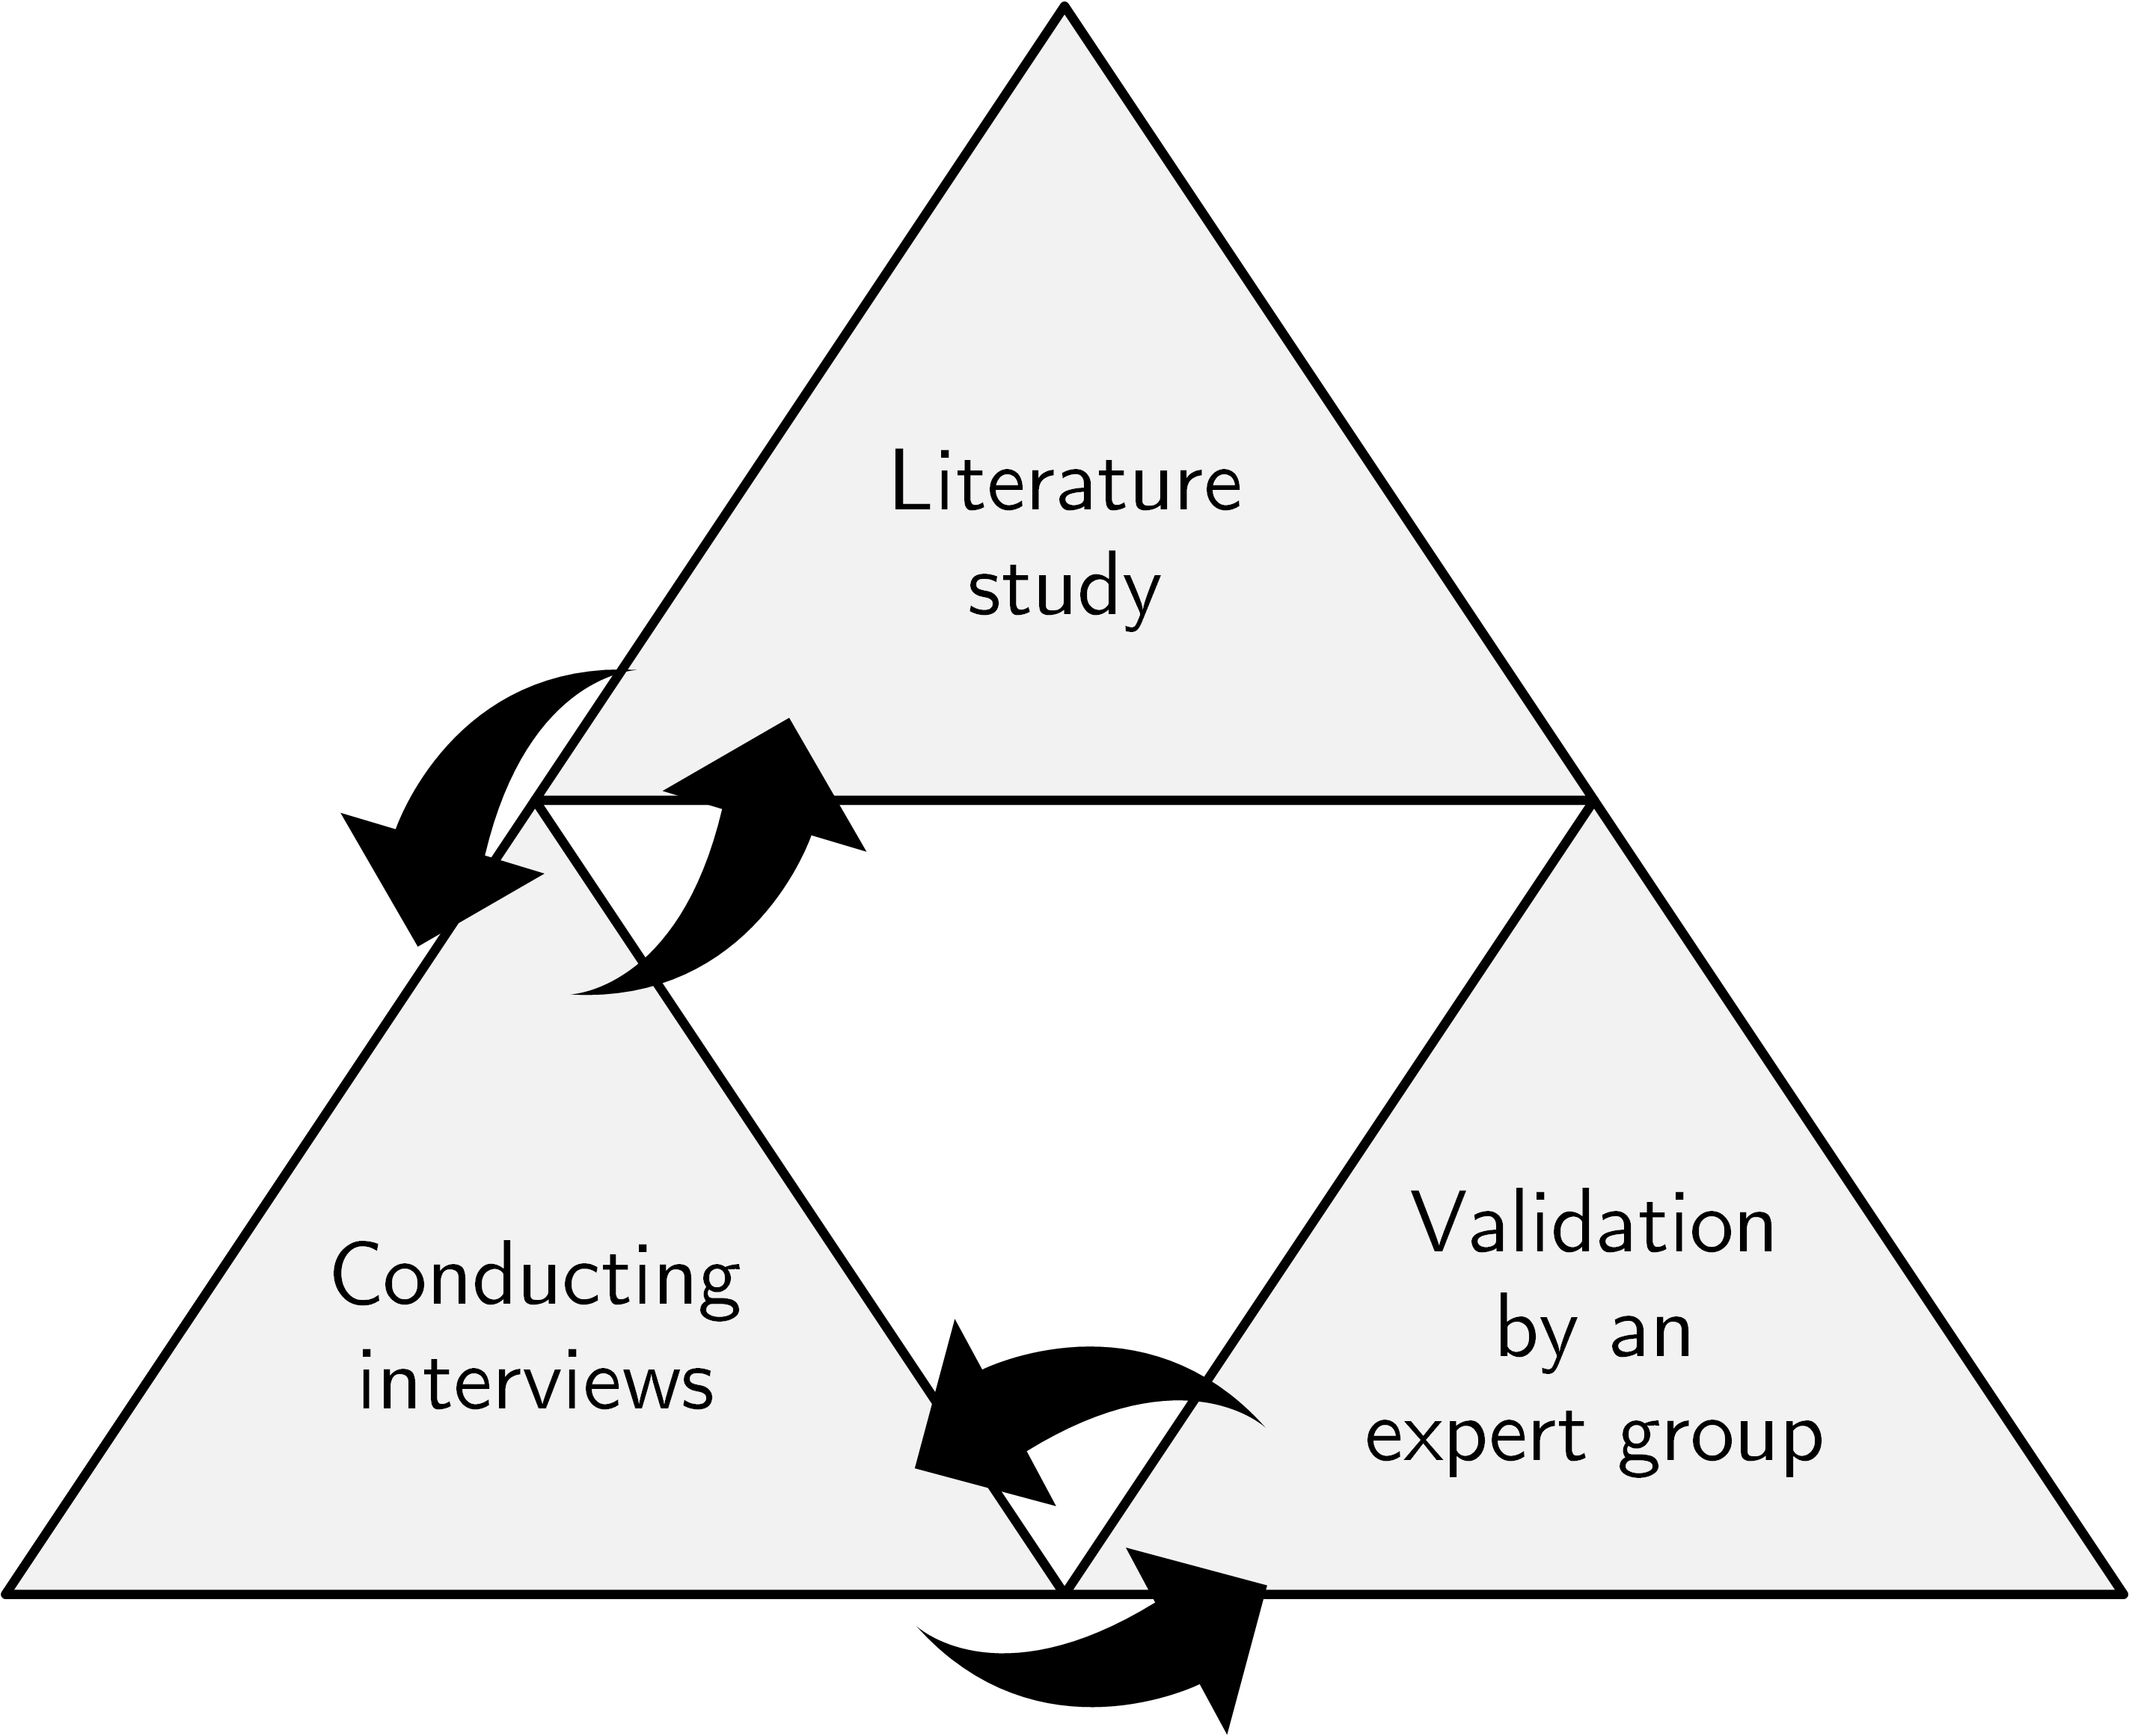
\includegraphics[width=0.45\linewidth]{images/researchmodel}
	\caption[Research model]{Research model}
	\label{fig:researchmodel}
\end{figure}

\section{Research approach}
\label{sec:researchapproach}
How will we conduct the literature study, interviews, and the validation with an expert group? This question is what this section will answer. This section describes the approach in detail to make the research replicable.
\subsection{Literature study}
\label{sub:literaturestudy}
The literature study answers the first five sub-question \cref{sec:introresearchquestion} of this research. We use specific keywords to find literature in online scientific libraries. The online scientific libraries we use are Web of Science, Researchgate, Google Scholar, and Semantic Scholar. We use the full name and the abbreviation of the concept to search for literature. E.g. \acrlong{ea} and \acrshort{ea}. Literature is accepted if it complies with quality \glspl{attribute}. These quality \glspl{attribute} are accuracy, authority, objectivity, currency and coverage \parencite{CityUniHongKong2021}. For currency, we assessed if the information is current and that it was published. We used a rule of thumb of 15 years to be current. For coverage, we assess the literature on relevance. The literature must be on the concept itself, but there must be a link with one or more concepts of this research. For replicability and reusability, we administrate the found literature.

\subsubsection{System}
\label{subsub:system}
We use two key literature sources for the system concept. These two sources are \textcites{Ackoff1973}{Gharajedaghi2011}. \textcite{Gharajedaghi2011} is one of the authors recognised by \textcite{Lapalme2012} as a follower of the \acrlong{ea} school of thought of \gls{enterpriseecologicaladaptation}. \textcite{Ackoff1973} was one of the pioneers of modern systems science. He used the work of  \textcite{Bertalanffy1968}, who coined systems theory in 1940 \parencite{Systemstheory2022}, as a base for his research. We researched citations on the works of \textcites{Ackoff1973}{Gharajedaghi2011} to start the literature study on system. We broaden the scope by using the following keywords for the online scientific libraries: \textit{system}, \textit{\gls{sos}}, \textit{\gls{sie}}, \textit{ecosystem}, \textit{\gls{antifragile} system}, and \textit{\acrlong{ea} system}.

\subsubsection{Antifragile}
\label{subsub:antifragile}
We use three key literature sources for the \gls{antifragile} concept. These two sources are \textcites{Taleb2012}{Botjes2020}{Botjes2021}. \textcite{Taleb2012} is the author who coined the concept of \gls{antifragile} while \textcite{Botjes2020} conducted extensive literature research on \gls{antifragility}. We use \textcite{Botjes2020} to find literature on antifragile. \textcite{Botjes2021} is an published article but misses the extensive reference to literature. \textcite{Botjes2021} is only used as literature and not as a source. We do not search for literature on \gls{antifragile} before July 2019, but only between July 2019 and April 2022. The research of \textcite{Botjes2021} ended in June 2019 so we only need literature after the research of \textcite{Botjes2021}. We used the same academic search engines and keywords as \textcite[p.~5]{Botjes2021}.

\subsubsection{Enterprise Architecture}
\label{subsub:enterprisearchitecture}
We use three sources to start the literature research. These sources are \textcites{Graves2008}{Hoogervorst2009}{Lapalme2012b}. Why these sources. The literature of these authors do align best with the concepts \gls{antifragile}, \gls{sos} and \gls{sie}. We use the following keywords for the online scientific libraries: \acrlong{ea}, \acrlong{ea} success factors, \acrlong{ea} \gls{antifragile} system, \acrlong{ea} ecosystem, \acrlong{ea} \gls{ps}, \acrlong{ea} \gls{sie}, \acrlong{ea} \gls{sos}.

\subsubsection{Public sector}
\label{subsub:publicsector}
We use two key references for the concept of public sector to start off the literature research. These two sources are \textcites{Wal2008}{Nurmi2021}. \textcite{Wal2008} compares the public and private sectors on core values while \textcite{Nurmi2021} researches the use of ecosystems in the public sector. We use the following keywords for the online scientific libraries: \gls{ps}, \gls{ps} \gls{antifragile}, \gls{ps} \gls{resilient}, \gls{ps} system, \gls{ps} ecosystem, \gls{ps} \gls{sos}, \gls{ps} \gls{sie}, \gls{ps} collaboration with the private sector, and \gls{ps} differences to the private sector.

\subsection{Interviews}
\label{sub:interviews}
We use semi-structured interviews to have the possibility to capture more information than a structured interview. The benefits of a semi-structured interview are that a semi-structured interview encourages two-way communication \parencite[pp.~87--88]{Recker2012}. We can validate our findings while at the same time we can collect new data. Furthermore, the interviewees may discuss sensitive issues more easily. We select interviewees from the public sector with a different profile than the expert group. The different profile helps with the triangulation of the research. We decided to use \glspl{cxo} for the interviews to get the business perspective of the public sector. We defined a set of topics for discussion. These topics are \acrlong{ea}, \gls{agility}, \gls{uncertainty}, unexpected events, risk appetite, \gls{diversity} and \gls{optionality}. We expect to cover all the attributes using the topics. The interviews are recorded and transcribed for future processing.

\subsection{Expert Group}
\label{sub:expertgroup}
The expert group will brainstorm for possible new \glspl{attribute}, discuss the \glspl{attribute}, and rate the \glspl{attribute}. The expert group is an qualitative tool. By using different tools, we strengthen the findings to be more reliable and valid \parencite[p.~91]{Recker2012}. We use a different perspective for the expert group members than for the interviewees. Instead of using a business perspective, we decide to use the \acrlong{ea} perspective of the Dutch \gls{ps}. A group support system supports the expert group session with the administration, reporting and needed tools. The expert group session is recorded and transcribed for future processing.

\subsection{Conclusion and discussions}
\label{sub:conclusionanddiscussions}
Before we can answer the research question, we combine the \gls{triangulation} results so we can sort and rate the \glspl{attribute}. An \gls{attribute} is most likely a success factor when the literature identifies the \gls{attribute}, the interviews confirm it, and the expert group agree with it. However, with this approach, we risk missing \glspl{attribute} that are specific to the \gls{ps}. These \glspl{attribute} can be essential distinguishing factors for the \gls{ps}. The \glspl{attribute} from the literature are not specific to the \gls{ps} but generic. We decided on an additional rule to overcome this shortcoming. An \gls{attribute} is likely a success factor when the \gls{attribute} meets two out of three requirements. \Glspl{attribute} that do not meet these two rules are not confirmed to be a success factor. This result gives us an answer to the main research question ''What are the success factors that positively influence the contribution of \acrlong{ea} in achieving \gls{antifragility} in the \gls{ps}?'' 

\section{Implementation of research quality}
\label{sec:researchqualityimplementation}
The research model is defined. But how do we ensure that this approach also fulfils our quality requirements? We have two sets of quality principles we want to fulfil. The principles of \textcite{Recker2012} and the FAIR principles of \textcite{GOFAIR2017}.

When we look at the principles of \textcite[pp.~15--17]{Recker2012} we have the principles replicability, independence, precision, and falsification. We ensure that the thesis contains a description of all steps. Steps taken for the literature study, the interviews, and the expert group.  To support replicability the used data sets are publicily available for use.

Replicability, independence, precision, and falsification are the principles \parencite[pp.~15--17]{Recker2012}. We ensure that the thesis contains a detailed approach for replication. The used data sets are made publicly available to support replicability. By rationalising everything, we remove as much subjectivity as possible. The output of the interviews and the expert group are normalised to remove possible bias from the system. This approach supports the principle of independence. Defining every concept supports the principle of precision. For every concept, there is a clear definition available. When there are more definitions, research is necessary. Using a rationale makes it clear why we did choose a particular definition. All the definitions are available in \cref{ch:theoreticalbackground} or the Glossary of Terms. Using discussions (\cref{sec:discussions}) helps with the falsification of this research.

Findable, accessible, interoperable, and reusable are the principles of FAIR \parencite{GOFAIR2017}. Keywords, links, structures, and metadata that can be indexed support findability. GitHub, Zenodo, and Researchgate publish the thesis and the used data sets. We created objects with a location for acquiring the source for sources that are not to be published publicly. Publishing based on Open Access supports the principle of accessibility. The principle that is least relevant for this research is interoperable. It is least relevant because this principle is mostly for quantitative methods. Nevertheless, the datasets are available as Microsoft Excel files for analysis. The files are easy to import, reuse, or combine in other environments to support the principle of reusability. The publication of the thesis and the used datasets use a Creative Commons license (\href{https://creativecommons.org/licenses/by-sa/4.0/}{CC-BY-SA 4.0}). The thesis and the used data sets can be shared and adapted as long as the original author is attributed and the possible derivate uses the same license.

\subsection{Research infrastructure and tooling}
\label{sub:researchinfraandtooling}
We describe how we worked with the tools we used to increase the quality of the research. We expect to increase replicability, findability, accessibility, interoperability, and reusability. We describe this in three subsections: the research execution, the administration and the creation.
\subsubsection{Research execution}
\label{subsub:tbresearchexecution}
For the administration of literature research, Apple Numbers\footnote{\url{https://apps.apple.com/us/app/numbers/id409203825}} is used. The administration is saved as a Microsoft Excel\footnote{\url{https://www.microsoft.com/en-us/microsoft-365/excel}} file for accessibility and reusability. The literature is administrated with the following columns: ID (for a unique ID per item), search terms used, scope, title, subtitle, author(s), year, type, Bib\LaTeX\ citation key, title relevance, abstract relevance, content relevance, found at, doi/isbn, url, date found, duplicate, date used, use for, and notes. Researchgate\footnote{\url{https://www.researchgate.net/}}, Web of Science\footnote{\url{https://app.webofknowledge.com/}}, Google Scholar\footnote{\url{https://scholar.google.com/}}, and Semantic Scholar\footnote{\url{https://www.semanticscholar.org/}} are the main sources for searching for literature. PaperPanda\footnote{\url{https://paperpanda.app/}} is used for hard to find literature. The literature administration is, together with the publicly available literature, stored in the repository of the master thesis\footnote{\url{https://github.com/JRBliekendaal/master-thesis/tree/main/literature}}. For non-public available literature, the administration contains the location where the literature is retrievable. We add the literature to a bib\LaTeX\ file for future reference. For traceability, the entries in the bib\LaTeX\ file contain the same Unique ID in the comments field. We work paperless. All the literature is in pdf or in ebook format. We use Acrobat Reader DC\footnote{\url{https://get.adobe.com/reader/}} and an Amazon Kindle Oasis\footnote{\url{https://www.amazon.com/dp/B07L5GJD99}} for reading. We use Microsoft Teams for interviews. We use the transcript and session recording functionality. The transcript and recordings contain sensitive information and are not publicly available. The transcripts and recordings are securely stored and are available upon request by the Antwerp Management School. We use QDA Data Minder Lite\footnote{\url{https://provalisresearch.com/products/qualitative-data-analysis-software/freeware/}} to label transcripts so that analysis can be done with Apple Numbers. For the Expert Group, Meetingwizard\footnote{\url{https://www.meetingwizard.nl/}} is used for brainstorming, surveys and rating. The Antwerp Management School supplies the license for using Meeting Wizard. The data set of the Meeting Wizard session is stored as a Microsoft Excel file in the repository of the thesis (anonymised).
\subsubsection{Research administration}
\label{sub:tbresearchadministration}
We use a non-public GitHub repository to store privacy-sensitive information. The same GitHub repository is used for staging thesis parts that still need to be anonymised. For note-taking, Leuchtturm1917\footnote{\url{https://www.leuchtturm1917.us/notebook-classic.html}} notebooks are used together with a mechanical pencil of Rotring\footnote{\url{https://www.rotring.com/rotring-600-mechanical-pencil-1/SAP_1904443.html}} and a Tombow Mono Zero eraser\footnote{\url{https://www.tombow.com/en/products/mono_zero/}}.
\subsubsection{Thesis creation}
\label{subsub:tbresearchcreation}
An Apple Macbook Air\footnote{\url{https://en.wikipedia.org/wiki/MacBook_Air_(Apple_silicon)}} with model number A2337 is used to write the thesis. We use the markup language \LaTeX\footnote{\url{https://www.latex-project.org/}} with the typesetting environment of MacTex\footnote{\url{https://www.tug.org/mactex/}} with the document type of ''Report'' from KOMA-Script\footnote{\url{https://ctan.org/pkg/koma-script}}. The editor TexStudio\footnote{\url{https://www.texstudio.org/}} is used with Bib\LaTeX\footnote{\url{https://ctan.org/pkg/biblatex/}} for managing references with the style of APA 7th Edition\footnote{\url{https://apastyle.apa.org/}}. We store the thesis files on Apple iCloud\footnote{\url{https://www.icloud.com/}} that is used by GitHub Desktop\footnote{\url{https://desktop.github.com/}} to synchronise with a public GitHub repository\footnote{\url{https://github.com/JRBliekendaal/master-thesis}}. GitHub\footnote{\url{https://github.com/}}  is used for source control and for reviewing and discussing the topics with the research organisation. The thesis source files are archived in zip format and copied to an Amazon S3 Blob\footnote{\url{https://aws.amazon.com/s3/}} for backup. We use a backup rotation of seven versions. Using MSP360 Explorer\footnote{\url{https://www.msp360.com/explorer/windows/amazon-s3.aspx}} helps us with storing backups. Grammarly\footnote{\url{https://www.grammarly.com}} (with a paid subscription) performs spelling, grammar, style, and plagiarism checking. Microsoft Visio Professional\footnote{\url{https://www.microsoft.com/en-ww/microsoft-365/visio/}} is used to create figures. The GitHub repository contains all the sources\footnote{\url{https://github.com/JRBliekendaal/master-thesis/tree/main/images/sources}}.